\section{Research Themes}

\begin{figure}
  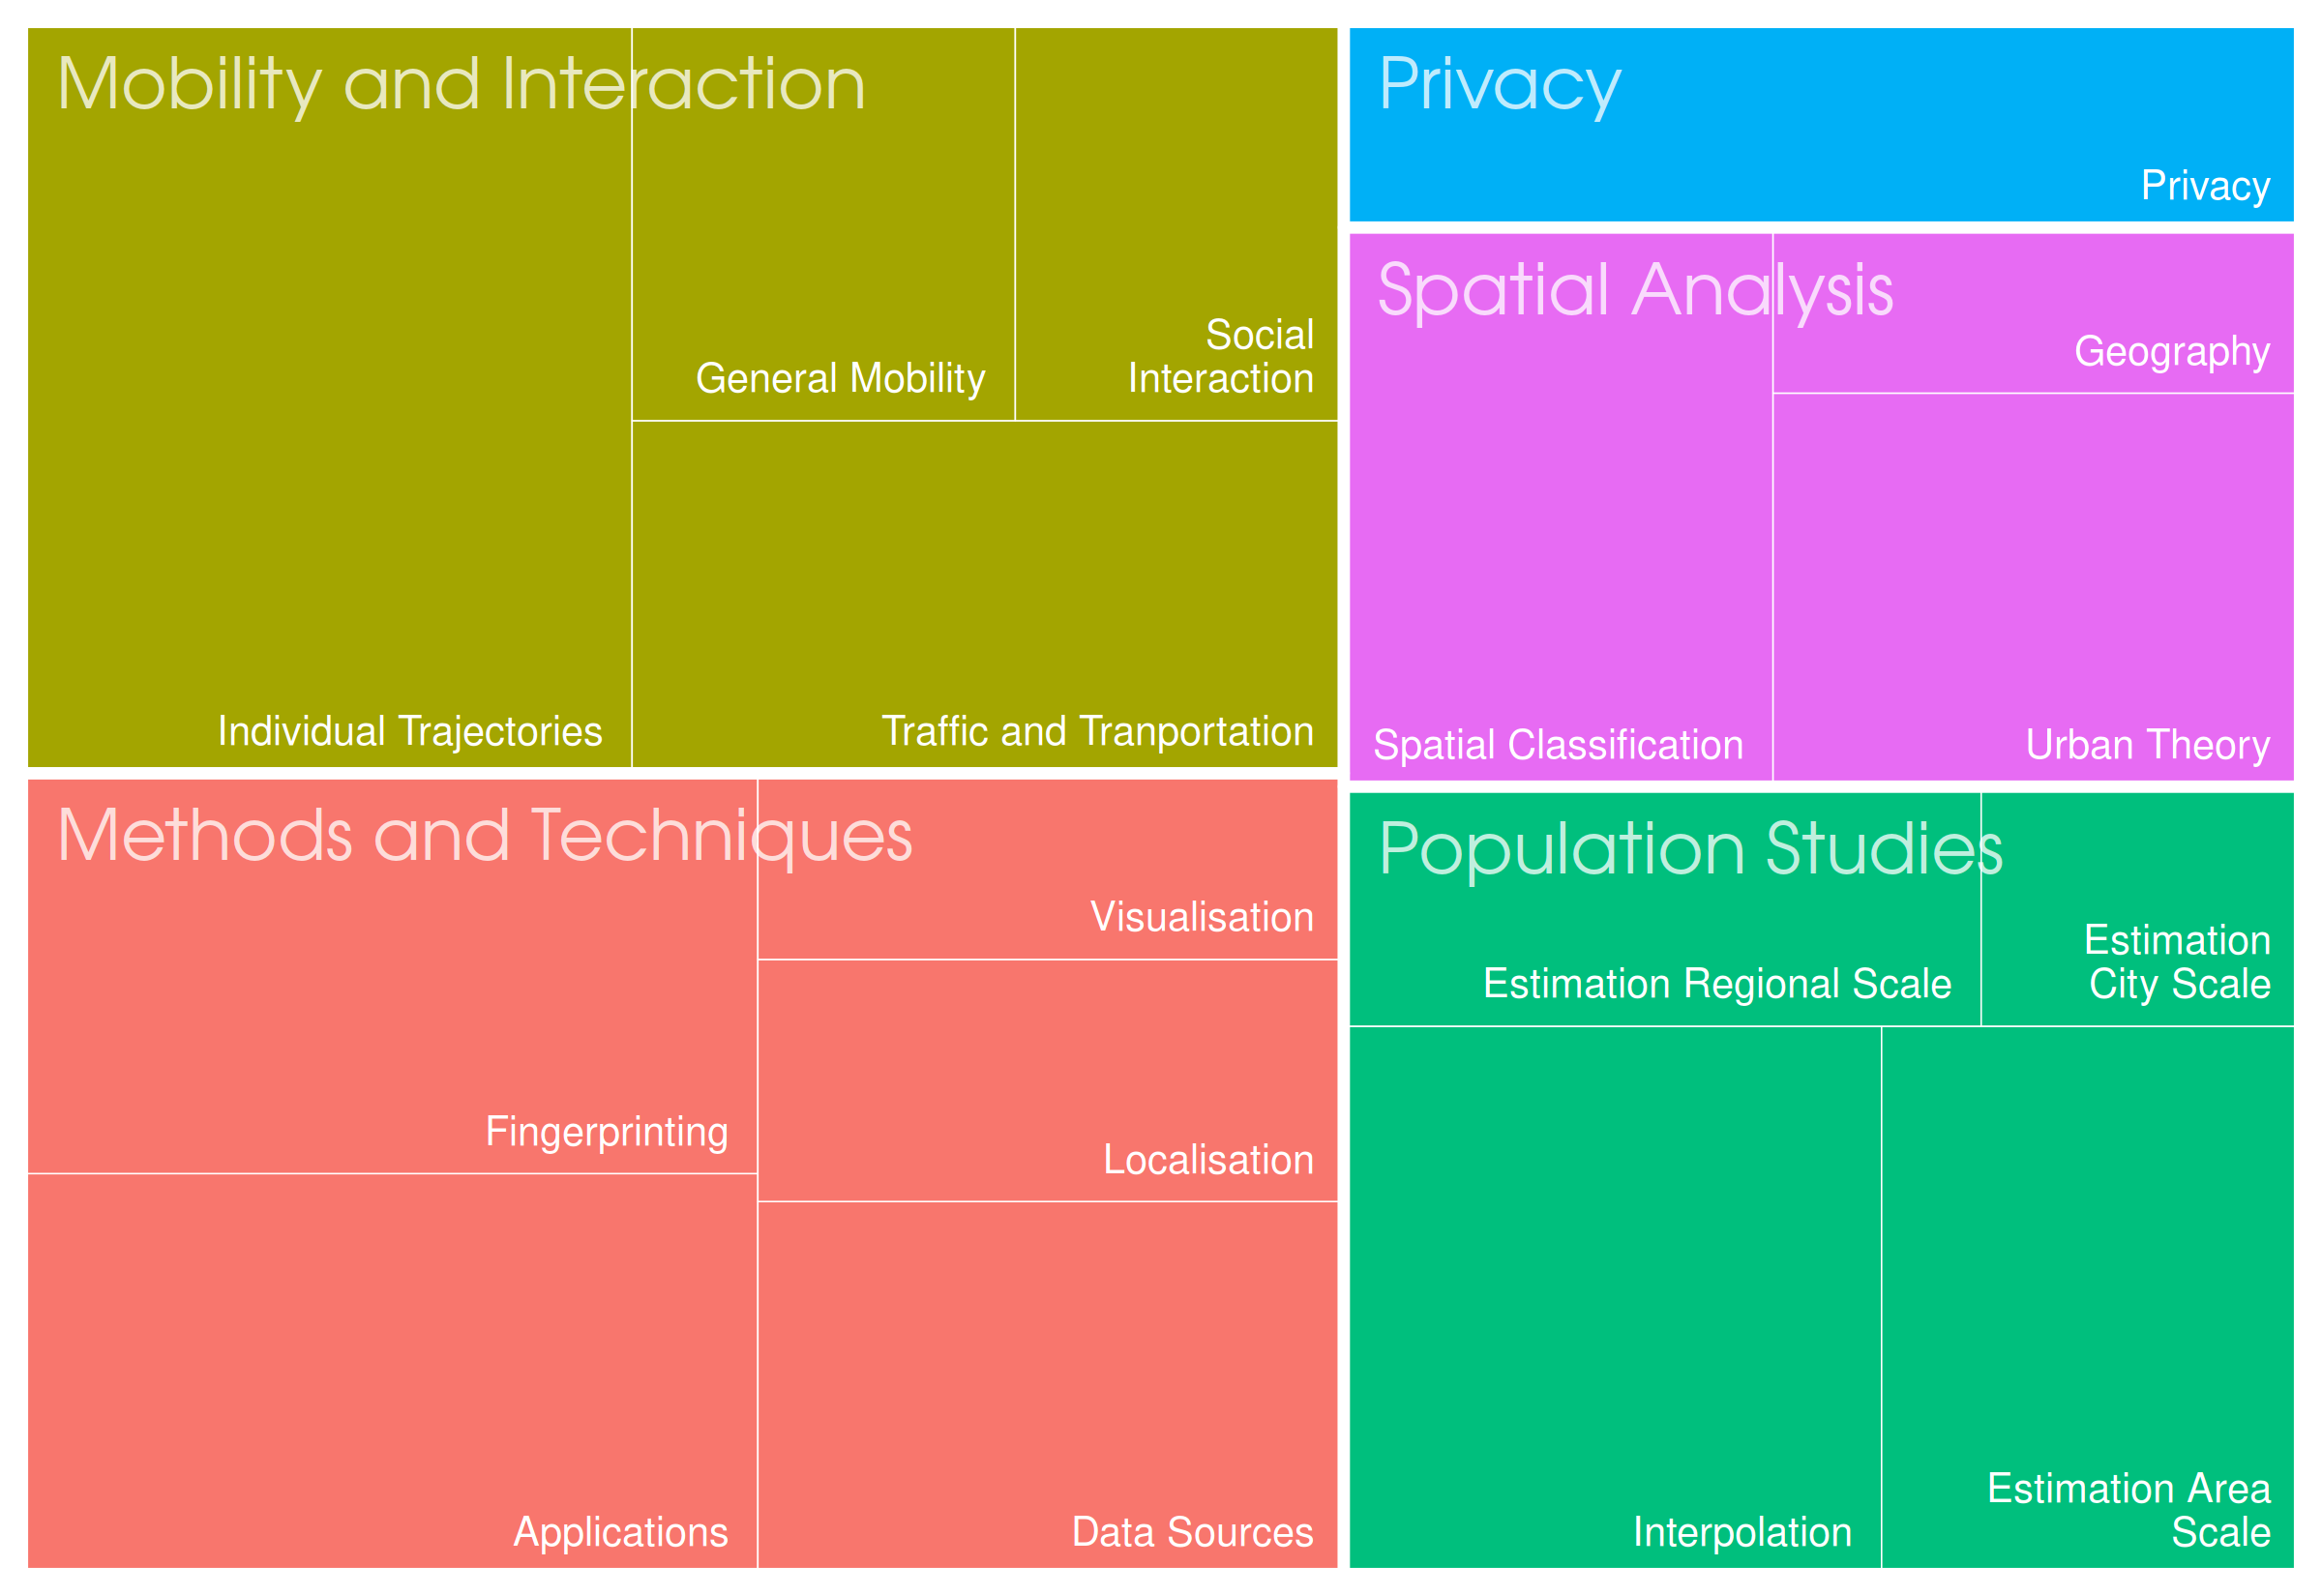
\includegraphics{images/literature-themes-treemap.png}
  \caption{Tree-map showing the volume of research conducted under each major themes and their sub-themes.}
  \label{figure:literature:themes}
\end{figure}

In this section we look at the major themes and questions tackled by this knowledge base.
We start by classifying the research into the major and minor themes explored in them as shown in Figure \ref{figure:literature:themes}.
The tree-map shows the volume of research in corresponding themes measured in terms of number of publications.
We can observe that the research is conducted in five major areas - population studies focussing on the creating and utilising data on distribution and nature of human activity, mobility and interaction focussing on the changes in these distributions, understanding the nature and function of space from these distribution and change, methods and techniques which can be used to conduct the research and finally issues and solutions related to the privacy of the users while conducting these research.
We can also observe that most of the research conducted are in the domain of mobile and social interaction closely followed by the population distribution.
In the following sections we discuss these in detail along with their sub themes with the following framework,

\begin{enumerate}
  \setlength{\itemindent}{2em}
  \itemsep-0.25em
  \item What are the major lines of questioning?
  \item What has been done previously?
  \item Where are the opportunities for further research?
\end{enumerate}

\subsection{Population Studies}
Though \citet{foley1954} and \citet{schmitt1956} started this line of research in 1950's with the discussion on estimating daytime population using broader datasets it was not until the 80s significant volume of research kicked off in this area of study.
From 80s until mid 2000's numerous studies were conducted on measuring and studying the population at a granular level both spatially and temporally.
The focus of the research around this time was primarily on interpolation from the larger datasets created using censuses, regional or national level sample surveys and other centrally collected sources of data.
There have been numerous fairly successful attempts with methodologies where a broad dataset such  as regional level population summaries and modelling or interpolating more granular data from them by augmenting with other sources of data such as street networks\cite[-10cm]{reibel2005}, remote sensing\cite[-6.5cm]{sutton1997} \cite[-3.5cm]{yuan1997} \cite{chen2002} etc.
\citet{dobson2000, dobson2003a, bhaduri2002, bhaduri2007} and \citep{mennis2003, mennis2006} are examples of such research methodology.
These studies were almost done on a city scale or above with mostly modelling or interpolation methods since the data sources were few and were centrally collected.

Around 2005, there was a sharp shift in research where the interpolation methods were replaced by highly available granular data collected over cellular network.
Studies were conducted on estimating population densities, presence of tourists, general activity pattens using data from cellular networks.
Most of these research were conducted at a far larger geographic scale looking at things at an area level \citep{pulselli2008,girardin2009,phithakkitnukoon2010,yuan2016}.
There were efforts in using device level sensors such as global positioning system(GPS), Wi-Fi and Bluetooth to detect population distribution and socio-geographic routines \citep{calabrese2010,rose2010,farrahi2010}.
There have been studies on looking at people distribution as granular as queue lengths as discussed by \citet{wang2013} to city level dynamic population mapping where the limitations of traditional datasets generated through censuses and surveys \cite[-4cm]{deville2014}.

Around the 2015, along with the data collected directly from the mobile devices,the data that are generated by the users activity on these devices are became more important.
Social media data such as twitter \citep{lansley2016} and other consumer data such as loyalty cards \citep{lloyd2018}, smart cards \citep{ordonez2012} etc. have also become a significant sources of data for such research.
Recently, with increased concerns and legislation on privacy, there have been studies which go back to the effort of interpolating granular data from broader datasets but using more data and processor intensive technologies such as agent based modelling\cite[-2.5cm]{crols2019}, deep learning, etc.\cite{shibata2019}.
Though there have been a lot of work done in most of the directions in this research area, the clear gap arises due to the absence of a continuous granular and sufficiently longitudinal data-sets to complement the methodologies that have been developed. 

%==============================================================================%
% Rao, 2015
% yuan 1997, 2016
%==============================================================================%

\subsection{Human Mobility and Interaction}
Urban mobility research significantly benefited from the decentralised collection of granular data (Castells, 2000) and its augmentation through traditional models of travel behaviour (Janssens, 2013).
The large volume of research done under these themes is discussed in detail in the section on techniques and technologies.

\subsection{Methodology and Techniques}
Visualising the temporal dynamics of data collected on human activities through decentralised processes poses significant challenges when approached with traditional cartographic concepts (MacEachren, 2001 Hallisey, 2005).
Digital media especially animation has been explored as an option to solve for the temporal dimension (Morrison, 2000; Lobben, 2003) but is bound by the cognitive limits of the viewer (Harrower, 2007).
There have been approaches proposed around animations of generated surfaces (Kobayashi, 2011) and network-based visualizations (Ferrara, 2014) leaving gaps in research for new methods in dynamic geo-visualisation (Fabrikant, 2005) and visualising path and flow of phenomena (Thomas, 2005).
This provides us with a promising opportunity for research in methods for visualising high frequency, hyper-local pedestrian data within the limits of cognition of the viewer.

\subsection{Spatial Analysis Theory and Modelling}
Traditional and modern geography were usually dominated by the study of centrally collected data acquired through extensive field surveys and remote sensing.
In the last two decades, a significant paradigm change has been introduced by the availability of unprecedented amount of data generated by unconventional sources such as mobile phones, social media posts etc.
This move to the postmodern geography (Soja, 1989) has been accompanied by a change in our understanding of the built environment and human geography, from a static point of view to a more dynamic definition based on the bottom up mechanisms which manifest in them, such as economic activity and information exchange (Batty 1990, 1997, 2012, 2013a,b).
This transition into the digital age (Graham, 1999; Tranos, 2012; 2013) has changed the politics of space and time (Massey, 1992) and been more pronounced in the study of urban built environment where technology has redefined the concepts of place and space (Graham, 2001; Sassen, 2001; Graham, 2002).
With the ability to collect and analyse of data on large complex systems in real-time (Graham, 1997), we are exploring the possibilities of understanding their structure and organisation using concepts of complexity theory (Bettencourt, 2013; Portugali, 2012) with more emphasis on their temporal patterns such as the argument towards finding the pulse of the city (Batty, 2010).
With the population getting more and more connected (Castells, 2010), the nature of space/place is being dynamically defined by the population themselves (Giuliano, 1991) and vice versa (Zandvliet, 2006).
This movement to the digital era was accompanied not only by optimism in its potential (Thomas, 2001; Nature, 2008) but also by the questions raised on the challenges in handling the diverse, large scale, non standardised data (Miller, 2010; Arribas-Bel, 2014 a) it produces and the usefulness or representativeness of the resulting analysis.
Nonetheless, availability of such data has impressive uses in urban studies (Bettencourt, 2014) especially with advancement of new technologies (Steenbruggen, 2015) and possibility of distributed, crowdsourced data collection (Lokanathan, 2015).

\subsection{Privacy}
The rise in personal technology has many opportunities for researchers and industry but at the same time has increased the general concern on privacy (Saponas, 2007; Krumm, 2009).
There is immense value in uniquely identifying and profiling information on people for specific purposes such as security (Cutter, 2006) and law enforcement (Dobson, 2003) but also has extreme risks associated when not handled with care (VanWey, 2005).
Strictly protecting personal information while ensuring the information is usable for research by maintaining the uniqueness in the data is the major concern which leads us to frameworks for secure practices in confidentially collecting and using the location data (Duckham, 2006; Tang, 2006; Lane, 2014).
Some efforts seek to accomplish this through cryptographic hashing algorithms (Pang, 2007) while others aim to thwart identification and tracking at the device level by techniques such as MAC randomisation (Gruteser, 2005; Greenstein, 2008).
The consent of users’ for the collection and use of such information from their mobile devices is low but with smart devices becoming ubiquitous there is a significantly improved acceptance when the process offers value in return such as discounts and monetary benefits (Kobsa, 2014) .

\begin{figure*}
  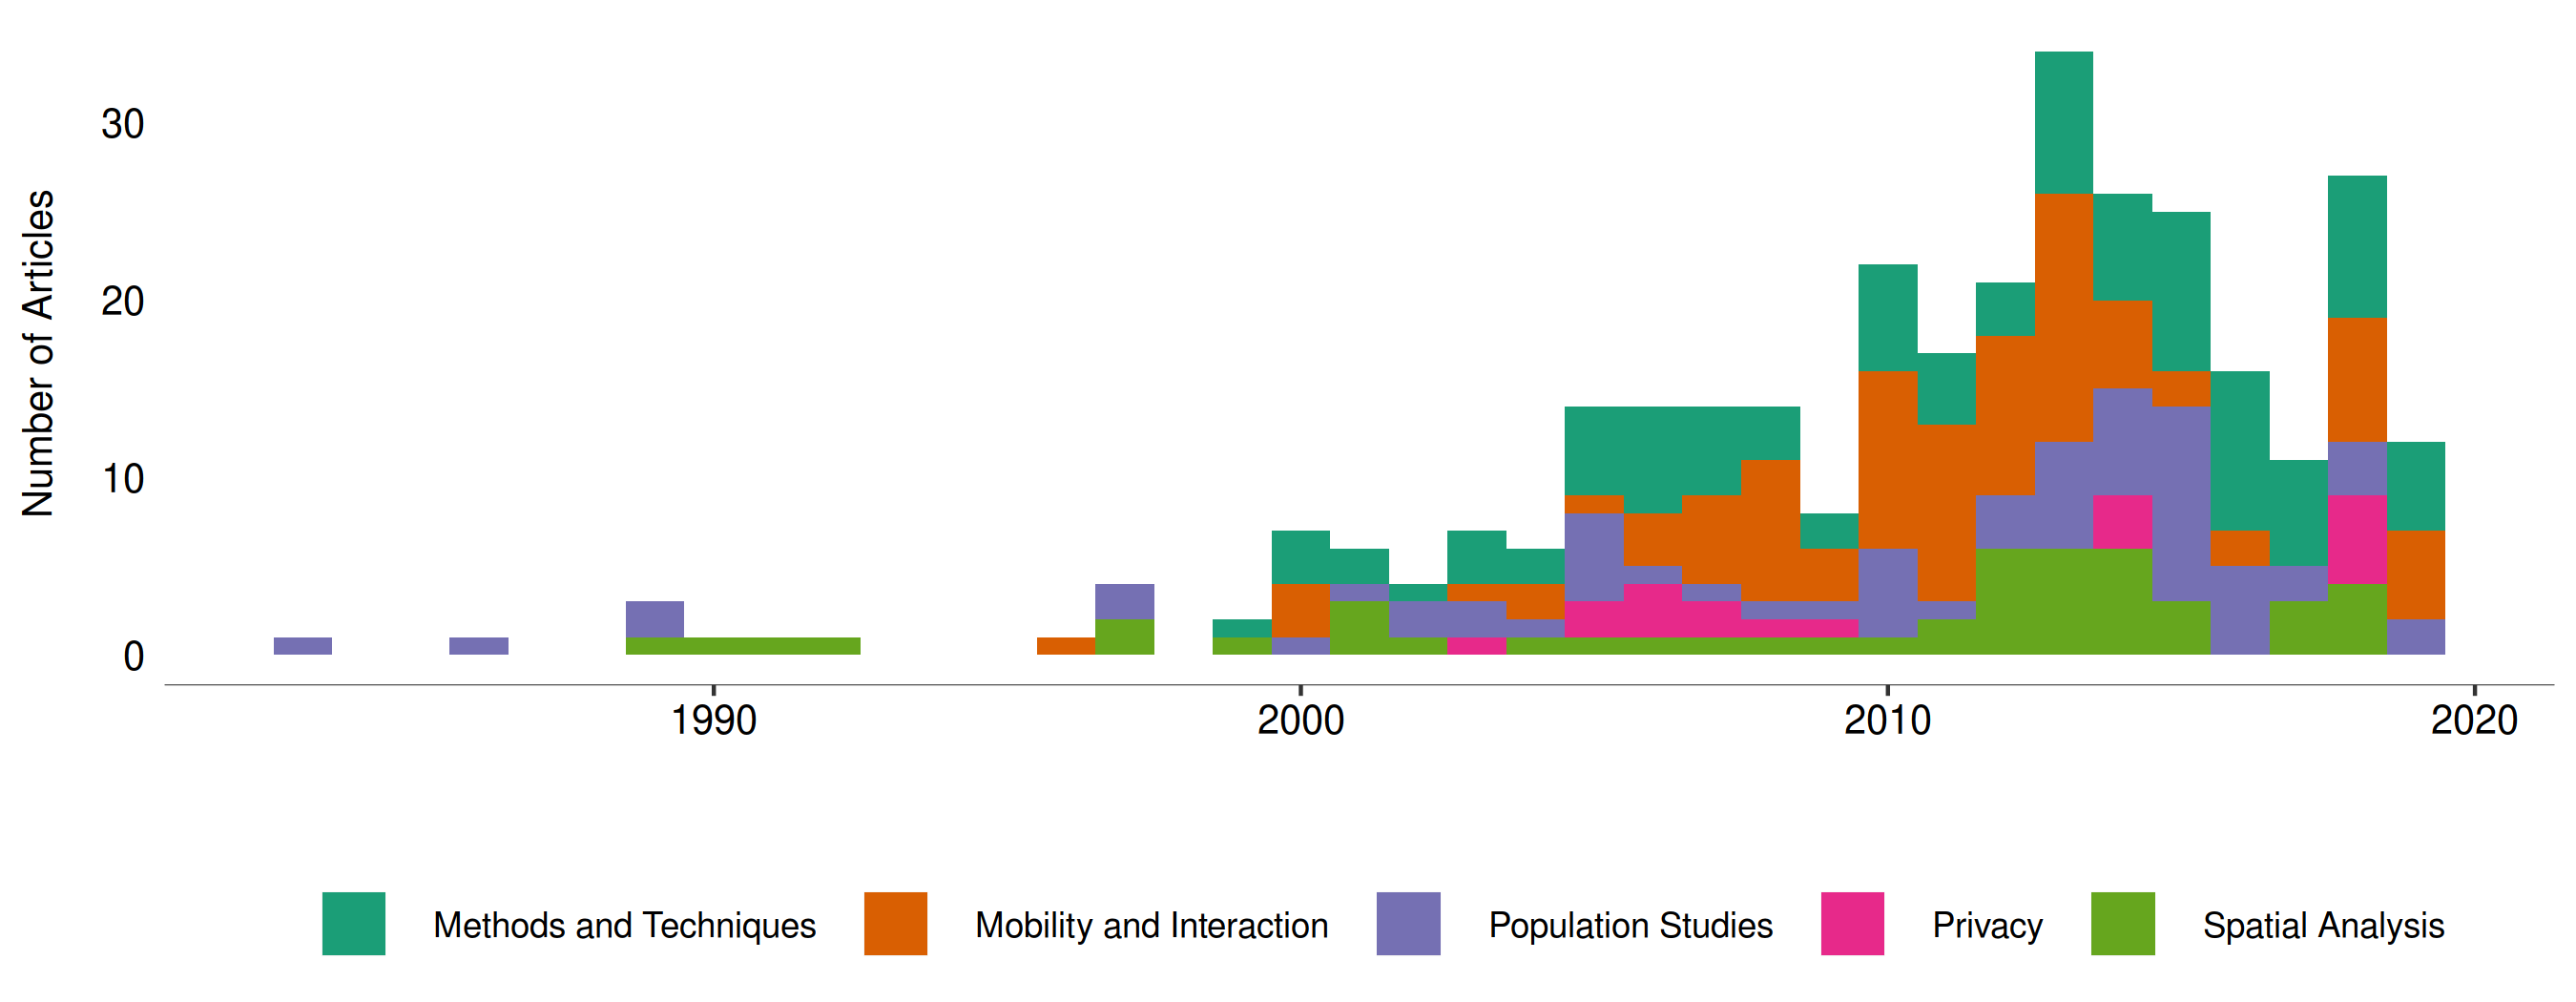
\includegraphics{images/literature-themes-timeline.png}
  \caption{Outline of the `Medium data toolkit' devised to collect, process, visualise and manage the Wi-Fi probe requests data}
  \label{figure:literature:themes:timeline}
\end{figure*}

\section{Research Trends}

Figure 1 shows the volume of research done in this topic since 1980 categorised based on their major themes discussed above.
We can observe that there are distinct trends in the research over time, with the explosion of interest in the last decade.
The research was mostly centered around population studies on interpolating larger datasets.
The period between 1990-2000 there was interest in potential of the new data generated by the digital age this coincided with mobile phones becoming more popular and ubiquitous with population in urban areas.
The next 5 years equal interest is observed in applying the data for population and urban mobility studies and in the development of theory, methods to use the data.
Between 2005 and 2010 the ‘mobile era’ saw significant rise in the volume of research, especially research focused on urban mobility and localisation and identification of the unique devices from the massive cellular network data which was met with an equal interest in privacy and data security.
In 2010 there was a clear increase in the volume of the research concerned with urban mobility, especially on tracking devices for trajectories.

This might be due to the emergence and proliferation of ‘smartphones’ around that time, which made collecting data from these devices directly much easier and less reliant on carrier provided datasets.
We also observe a focus on inferring the nature of the spaces these devices occupy and the social interactions between those who own these devices.
With the theoretical limit to predictability in human mobility quantified, the focus on urban mobility has been declining in the past few years.
This has been replaced by a renewed interest in population studies at a real-time, hyper-local level.
We also see a recent increase in interest in de-anonymisation in response to the industry adopting anti-tracking mechanisms in their products for example MAC randomisation in iOS devices.
Currently the research interest and gaps in the field concern the hyper-local estimation of population and nature along with methods to identify unique devices at this scale.
